\section{The adjoint-domain condition in the original weighted sequence
coordinates}\label{the-adjoint-domain-condition-in-the-original-weighted-sequence-coordinates}

Private continuation of NHR, 2026-09-25. Source: S. Waleed Noor,
\href{https://arxiv.org/abs/1809.09577v4}{arXiv:1809.09577v4}, native
author TeX §§1--5, byte-verified as recorded in
\texttt{SOURCE\_RECEIPT.json}. This note supplies direct proofs of the
isometry and all receiving maps it uses; it does not rely on an unread
book for the isometry. No publication, source-owner edit,
spectral-synthesis claim or RH conclusion is made.

\subsection{NAD0. Input retained}\label{nad0.-input-retained}

The input weights and maps remain exactly \[
 \omega_n=\frac1{n(n+1)},\quad
 \ell^2_\omega=\left\{a:\sum_{n\ge1}|a(n)|^2\omega_n<\infty\right\},
 \quad\Psi a(z)=\sum_{n\ge0}a(n+1)z^n,
\] \[
 Tf(z)=\frac{((1-z)f(z))'}{1-z},\qquad\Phi=T^{-1}\Psi.
\] All inner products are linear in the first variable. The weighted
Bergman space here has the precise coefficient norm
\(\|\sum b_jz^j\|_{\mathcal A}^2=\sum |b_j|^2/[(j+1)(j+2)]\). The map
\(\Psi\) is therefore isometric by its coefficients; no area-measure
convention is required for this proof.

These are arithmetic coefficient spaces \emph{after} the original
reconstruction. They neither assign parity to \(\tau\) nor construct
addition on it. The prior retraction of \(\tau+\tau=\tau\) remains in
force. The original \(Q=\mathcal B/I\), its full zero divisor, support
labels and raw dilations remain unchanged. This is a calculation on the
NHR receiver, not an identification of that receiver with all of \(Q\).

\subsection{NAD1. A direct complete-column proof of the
isometry}\label{nad1.-a-direct-complete-column-proof-of-the-isometry}

Let \(e_j(z)=z^j\) be the Hardy coefficient basis. In weighted sequence
coordinates the columns of \(T\) are \[
 v_0(n)=-1\quad(n\ge1),
\qquad
 v_m(n)=\begin{cases}0&n<m,\\m&n=m,\\-1&n>m,\end{cases}
 \quad(m\ge1).
 \tag{NAD1.1}
\] To verify the formula, differentiate \((1-z)z^m\), divide by \(1-z\),
and read the coefficient of \(z^{n-1}\). Thus \(T e_m=\Psi v_m\),
including the negative sign at \(m=0\).

The exact telescoping weight identities give \[
 \|v_0\|_\omega^2=\sum_{n\ge1}\frac1{n(n+1)}=1,
\] \[
 \|v_m\|_\omega^2=\frac{m^2}{m(m+1)}+
       \sum_{n>m}\frac1{n(n+1)}=\frac m{m+1}+\frac1{m+1}=1.
\] For \(0\le j<m\), the only common nonzero coordinates are \(n=m\) and
\(n>m\), and hence \[
 \langle v_j,v_m\rangle_\omega
 =-\frac m{m(m+1)}+\sum_{n>m}\frac1{n(n+1)}=0.
 \tag{NAD1.2}
\] Every sum converges absolutely. For an arbitrary
\(a\in\ell^2_\omega\), each weighted tail also converges absolutely by
Cauchy--Schwarz and \(\sum_{n\ge m}\omega_n=1/m\).

For completeness, suppose \(a\) is orthogonal to every column.
Orthogonality to \(v_0\) gives \(\sum_{n\ge1}a(n)\omega_n=0\), and
orthogonality to \(v_m\), \(m\ge1\), gives \[
 \frac{a(m)}{m+1}=\sum_{n>m}\frac{a(n)}{n(n+1)}.
\] Using the equation at \(m+1\) to expand the right side proves
\(a(m)/(m+1)=a(m+1)/(m+1)\). Thus \(a\) is constant. Its equation
against \(v_0\) then makes that constant zero. The columns are a
complete orthonormal basis.

It follows that the coefficient extension \(T:H^2\to\mathcal A\) is an
isometric isomorphism. It is the original analytic differential
expression, not only an abstract extension: for each fixed output
coefficient, the differential expression uses finitely many input
coefficients, so the polynomial identity passes to every \(H^2\)
coefficient limit. The resulting weighted sequence defines a holomorphic
function in the disk, since \(|a(n)|\le\sqrt{n(n+1)}\|a\|_\omega\).

This proves both the isometry and its surjectivity independently of the
book cited by Noor. The inspected human source remains the provenance
for selecting this particular map.

\subsection{NAD2. Exact inverse, weighted tails, and the sign of the
unit}\label{nad2.-exact-inverse-weighted-tails-and-the-sign-of-the-unit}

For \(a\in\ell^2_\omega\) set \[
 A_m(a)=\sum_{r=m}^{\infty}\frac{a(r)}{r(r+1)},\qquad
 H_a(m)=m A_m(a)\quad(m\ge1),\qquad H_a(0)=0.
 \tag{NAD2.1}
\] The complete-column expansion just proved gives
\(\Phi a(z)=\sum_{m\ge0}c_mz^m\), with \[
 c_0=-A_1(a),\qquad
 c_m=\frac{a(m)}{m+1}-A_{m+1}(a)
     =H_a(m)-H_a(m+1)\quad(m\ge1).
 \tag{NAD2.2}
\] The same last expression holds at \(m=0\) under the stated
\(H_a(0)=0\). In particular, \[
 \boxed{\sum_{m=0}^{N}c_m=-H_a(N+1).}
 \tag{NAD2.3}
\] No ordinary infinite tail of the \(c_m\) is asserted. The weighted
tails in NAD2.1 \emph{do} converge absolutely. Moreover \[
 |H_a(m)|\le\sqrt m\left(\sum_{r\ge m}|a(r)|^2\omega_r\right)^{1/2}
 =o(\sqrt m).
 \tag{NAD2.4}
\] The exact inverse recovery at every integer is \[
 a(m)=(m+1)H_a(m)-mH_a(m+1).
 \tag{NAD2.5}
\] For the source constant \(a(n)=1\), \(A_m=1/m\), \(H_a(m)=1\) and
\(c_0=-1,c_{m\ge1}=0\). Thus the full convention is \[
 \boxed{\Phi\boldsymbol1=-1.}
 \tag{NAD2.6}
\]

\subsection{NAD3. The adjoint domain is a weighted-tail
condition}\label{nad3.-the-adjoint-domain-is-a-weighted-tail-condition}

Let \(S\) be the Hardy shift, \(B=I-S\), and \(M=B^{-1}\) on
\(\operatorname{ran}B\). The operator \(B\) is injective;
\(\ker B^*=0\), because an \(\ell^2\) coefficient sequence fixed by the
backward shift is a constant sequence and hence zero. Thus
\(\operatorname{ran}B\) is dense and the adjoint \(M^*\) is defined.
From the adjoint definition itself, \[
 \operatorname{dom}M^*=\operatorname{ran}(I-S^*),\qquad
 M^*((I-S^*)d)=d.
 \tag{NAD3.1}
\] Indeed testing on \(Bf\), \(f\in H^2\), gives
\(\langle MBf,y\rangle=\langle f,y\rangle=\langle Bf,d\rangle\) exactly
when \(y=B^*d\).

The equation \(c_m=d_m-d_{m+1}\), combined with NAD2.3, has the unique
possible form \[
 d_m=d_0+H_a(m)\quad(m\ge1).
\] It is square-summable exactly when there is a scalar \(\ell\) such
that \[
 \boxed{\sum_{m=1}^{\infty}
 \left|m\sum_{r=m}^{\infty}\frac{a(r)}{r(r+1)}-\ell\right|^2<\infty.}
 \tag{NAD3.2}
\] Then \(d_0=-\ell\), \(d_m=H_a(m)-\ell\), and
\(\ell=\lim_{m\to\infty}H_a(m)\); uniqueness follows because a nonzero
constant sequence is not in \(\ell^2\). Consequently \[
 \mathfrak D_\omega:=\Phi^{-1}\operatorname{dom}M^*
 =\{a\in\ell^2_\omega:\text{NAD3.2 holds for a scalar }\ell\}.
 \tag{NAD3.3}
\] This is the explicit arithmetic sequence condition, with the original
weights and all constants retained. It is strictly stronger than
boundedness or convergence of the weighted tail averages alone.

Here is an exact witness for the last assertion. Put \(h_m=m^{-1/2}\)
and \(a(m)=(m+1)h_m-mh_{m+1}\). The mean-value estimate for \(x^{-1/2}\)
gives \(0<a(m)\le3/(2\sqrt m)\), so \(a\in\ell^2_\omega\). Its weighted
tail telescopes to \(A_m=h_m/m\), since \(h_m/m\to0\); hence
\(H_a(m)=m^{-1/2}\to0\). Nevertheless
\(\sum_m|H_a(m)|^2=\sum_m1/m=\infty\), so it fails NAD3.2. This is a
fully specified sequence calculation, not a proposed zeta zero.

For clarity, the exact local-Dirichlet interpretation is also retained.
The coefficient identity \[
 (I-S^*)d=d_0+(z-1)S^*d
\] and Noor's §1.3 characterization imply \[
 (\Phi a)^*(1)=-\ell,
 \qquad \mathcal D_{\delta_1}(\Phi a)=
 \sum_{m\ge1}|H_a(m)-\ell|^2.
 \tag{NAD3.4}
\] The exact adjoint-output norm, which includes the boundary
coefficient, is \[
 \boxed{\|M^*\Phi a\|_{H^2}^2
 =|\ell|^2+\sum_{m\ge1}|H_a(m)-\ell|^2.}
 \tag{NAD3.5}
\] This is the actual norm of the adjoint output, not a replacement for
the original ambient \(\ell^2_\omega\) norm.

\subsection{NAD4. A complete parameterization, not an implicit
inverse-image
notation}\label{nad4.-a-complete-parameterization-not-an-implicit-inverse-image-notation}

The condition has an equivalent explicit source parameterization: \[
 \boxed{\mathfrak D_\omega=
 \left\{a(m)=\ell+(m+1)e_m-me_{m+1}:\ell\in\mathbb C,
                   (e_m)_{m\ge1}\in\ell^2\right\}.}
 \tag{NAD4.1}
\] For a source already satisfying NAD3.2, this follows from NAD2.5 with
\(e_m=H_a(m)-\ell\). Conversely, for arbitrary \(\ell,e\) as displayed,
the resulting source lies in \(\ell^2_\omega\): the constant term has
squared weighted norm \(|\ell|^2\), and the two terms involving \(e\)
have bounded coefficient maps to that space, since \((m+1)/m\le2\) and
\(m/(m+1)\le1\). Summing the weighted tail gives exactly \[
 A_m(a)=\frac\ell m+
 \sum_{r\ge m}\left(\frac{e_r}r-\frac{e_{r+1}}{r+1}\right)
 =\frac{\ell+e_m}{m}.
\] The endpoint term tends to zero because \(e\in\ell^2\). Thus
\(H_a(m)=\ell+e_m\), proving the converse and the uniqueness of both
parameters.

The corresponding analytic function and exact ambient norm are \[
 \Phi a(z)=-\ell+(z-1)\sum_{m\ge0}e_{m+1}z^m,
\] \[
 \boxed{\|a\|_\omega^2=|\ell+e_1|^2+
               \sum_{m\ge1}|e_m-e_{m+1}|^2.}
 \tag{NAD4.2}
\] The latter follows from the direct isometry and NAD2.2, not from
removing either term. Meanwhile the norm of the adjoint output is
\(|\ell|^2+\sum|e_m|^2\), as in NAD3.5.

Even the adjoint itself has a full weighted-sequence formula. Write
\(\mathfrak M=\Phi^{-1}M^*\Phi\) on \(\mathfrak D_\omega\). Applying the
original column coefficient formula to \(d_0=-\ell,d_m=H_a(m)-\ell\)
gives \[
 (\mathfrak M a)(m)=mH_a(m)-\sum_{j=1}^{m-1}H_a(j)
 =\boxed{\frac12\left(m(m+1)\sum_{r\ge m}\frac{a(r)}{r(r+1)}
                     -\sum_{r=1}^{m-1}a(r)\right).}
 \tag{NAD4.3}
\] For the second equality, interchange a finite sum with the absolutely
convergent tails and use \(\sum_{j=1}^{q}j=q(q+1)/2\). The factor
\(1/2\), finite initial sum and infinite weighted tail are all retained.
Its squared \(\ell^2_\omega\) norm is precisely NAD3.5.

\subsection{NAD5. The raw cover becomes an exact weighted block
sum}\label{nad5.-the-raw-cover-becomes-an-exact-weighted-block-sum}

Retain Noor's \(W_n f(z)=(1+\cdots+z^{n-1})f(z^n)\). Define its adjoint
receiver in the weighted sequence coordinates by \[
 C_n=\Phi^{-1}W_n^*\Phi.
\] Since \((W_n^*c)_m=\sum_{r=0}^{n-1}c_{nm+r}\), the initial partial
sum through \(m-1\) is the initial partial sum of \(c\) through
\(nm-1\). Applying NAD2.3 and then NAD2.5 therefore proves \[
 \boxed{H_{C_na}(m)=H_a(nm),}
 \tag{NAD5.1}
\] \[
 \boxed{(C_na)(m)=n m(m+1)
       \sum_{r=nm}^{n(m+1)-1}\frac{a(r)}{r(r+1)}.}
 \tag{NAD5.2}
\] In particular \(C_n\boldsymbol1=\boldsymbol1\). The factor in NAD5.1
is \textbf{one}, not \(n\); the factor \(n\) remains in the full block
formula NAD5.2. The equality \(\|C_n\|=\sqrt n\) follows from the direct
isometry and \(W_n^*W_n=nI\). It is sharp, for example on \(W_n f\) in
Hardy coordinates. No cover operator is divided by \(\sqrt n\).

For a regular source NAD4.1 this action is particularly exact: \[
 \boxed{C_n:(\ell,(e_m)_{m\ge1})\longmapsto
                 (\ell,(e_{nm})_{m\ge1}).}
 \tag{NAD5.3}
\] Thus \(C_n\) preserves \(\mathfrak D_\omega\), its boundary value is
unchanged, and the actual local energy is \[
 \mathcal D_{\delta_1}(\Phi C_na)
 =\sum_{m\ge1}|e_{nm}|^2\le\sum_{m\ge1}|e_m|^2.
 \tag{NAD5.4}
\] The adjoint-output norm NAD3.5 also contracts. This does \textbf{not}
say that the ambient \(\ell^2_\omega\) norm contracts; its raw operator
norm is \(\sqrt n\). At the output level the exact intertwining is \[
 M^*W_n^*\Phi a=D_n M^*\Phi a,
 \qquad (D_nd)_m=d_{nm}\quad(m\ge0),
 \tag{NAD5.5}
\] which follows directly from \(W_n^*(I-S^*)=(I-S^*)D_n\). The notation
\(D_n\) here means this coefficient-subsampling operator only; it is not
the programme's source differential.

\subsection{NAD6. Full original jets and the raw original arithmetic
action}\label{nad6.-full-original-jets-and-the-raw-original-arithmetic-action}

For \(1/2<\Re s<1\), retain the NHR source vector \[
 a_s(r)=\frac{r(r+1)}{\bar s}
             \bigl(r^{-\bar s}-(r+1)^{-\bar s}\bigr).
\] Its absolutely convergent weighted tail telescopes, retaining every
factor, to \[
 A_m(a_s)=\frac{m^{-\bar s}}{\bar s},\qquad
 \boxed{H_{a_s}(m)=\frac{m^{1-\bar s}}{\bar s}.}
 \tag{NAD6.1}
\] For every full jet, with no simplicity assumption, \[
 H_{a_{\rho,j}}(m)=
 \left.\partial_{\bar s}^{j}\frac{m^{1-\bar s}}{\bar s}\right|_{s=\rho},
 \quad a_{\rho,j}=\left.\partial_{\bar s}^{j}a_s\right|_{s=\rho}.
 \tag{NAD6.2}
\] The Hilbert derivative bound from NHR2.2 justifies moving derivatives
through these continuous tail functionals. NAD5.1 now gives the full
action without an operator guess: \[
 C_na_{\rho,j}=n^{1-\bar\rho}
      \sum_{\ell=0}^j\binom j\ell(-\log n)^{j-\ell}a_{\rho,\ell}.
 \tag{NAD6.3}
\]

To state exactly where the original source acts, let \(E_+\subset Q'\)
be the finite span of original functionals
\(\varepsilon_{\rho,j}([F])=F^{(j)}(\rho)\) at actual right-off-line
zeros. The previously constructed conjugate-linear map is \[
 \mathcal A:=\Phi^{-1}\mathcal R:E_+\longrightarrow\ell^2_\omega,
 \quad\mathcal A\Bigl(\sum b_{\rho,j}\varepsilon_{\rho,j}\Bigr)
       =\sum\overline{b_{\rho,j}}a_{\rho,j}.
\] For the original \(U_n=nT_{1/n}\), whose multiplier is \(n^{1-s}\),
the exact comparison is \[
 \boxed{\mathcal A U_n'=C_n\mathcal A.}
 \tag{NAD6.4}
\] It uses the full Leibniz formula for all source jets, not an
identification of a primal dilation with an adjoint. The original zeta
pairing remains NHR3.1:
\(\langle h_k,\Phi a_s\rangle=(1-k^{1-s})\zeta(s)/s\). No completed zeta
or omitted gamma factor enters this route.

NAD6.1--6.2 make the earlier domain failure source-explicit: the
retained power-log tails cannot be a constant plus an \(\ell^2\)
sequence. The full finite-combination proof is NHR6, which did not
assume that individual terms cannot cancel; it proved that a nonzero
finite exponential-polynomial cannot become bounded in this strip.

\subsection{NAD7. An independent structural consequence of the
pullback}\label{nad7.-an-independent-structural-consequence-of-the-pullback}

There is a second exact proof that every nonzero finite received jet
combination is outside \(\mathfrak D_\omega\), now using the calculated
raw actions. Fix \(n>1\), and let \(V\) be a finite span of full jet
blocks with \(1/2<\Re\rho<1\). On this space every eigenvalue of \(C_n\)
is \(n^{1-\bar\rho}\), whose modulus is strictly greater than one. All
nilpotent terms are those in NAD6.3. Hence \(C_n|_V\) is invertible and
\((C_n|_V)^{-k}\to0\) in its finite-dimensional operator norm: each
inverse Jordan block is an exponentially decaying scalar times a
polynomial in \(k\).

For \(a\in V\cap\mathfrak D_\omega\), NAD5.3--5.5 imply \[
 \|M^*\Phi C_n^k a\|_{H^2}\le\|M^*\Phi a\|_{H^2}.
\] Since \(\Phi C_n^k a=(I-S^*)M^*\Phi C_n^k a\) and \(\|I-S^*\|\le2\),
the ambient norms \(\|C_n^k a\|_\omega\) are bounded. Consequently \[
 \|a\|_\omega
 \le\|(C_n|_V)^{-k}\|\,\|C_n^k a\|_\omega\longrightarrow0.
\] Thus \(a=0\). This proof keeps the original scalar eigenvalues and
the entire nilpotent action. It uses the genuine contraction of the
\emph{adjoint output}, not a false ambient contraction or a rescaled
cover.

The result strengthens the defect interpretation: the exact regular
source class is now parameterized by a scalar plus a weighted first
difference of an \(\ell^2\) sequence, and its raw transfer action is
coefficient subsampling. The complementary finite jets carry power-log
tails on which that same transfer grows. The mismatch is calculated in
the original receiving coordinates; it is not a claim that all programme
classes possess the regularity being tested.

No completeness theorem for all of \(\mathcal N^\perp\), no extension
from \(E_+\) to the full dual, no deletion of the opposite branch, no
equality with the original Weil pairing and no RH conclusion is
asserted. The exact full-source regularity condition has been derived
and tested; the global original return has not thereby been proved to
satisfy it.

\subsection{NAD8. Review and source
scope}\label{nad8.-review-and-source-scope}

An independent mathematical check verified the complete orthonormal
columns, the weighted inverse coefficients, the domain scalar's sign,
the block formula and the factor-one subsampling identity. The local
Dirichlet interpretation is the inspected Noor characterization; the key
isometry, inverse, adjoint-domain formula and raw action were directly
proved here. Earlier NHR source version/reading records remain valid.
This private continuation does not duplicate or modify the owner's GSP
spectral synthesis.

\begin{figure}
\centering
\pandocbounded{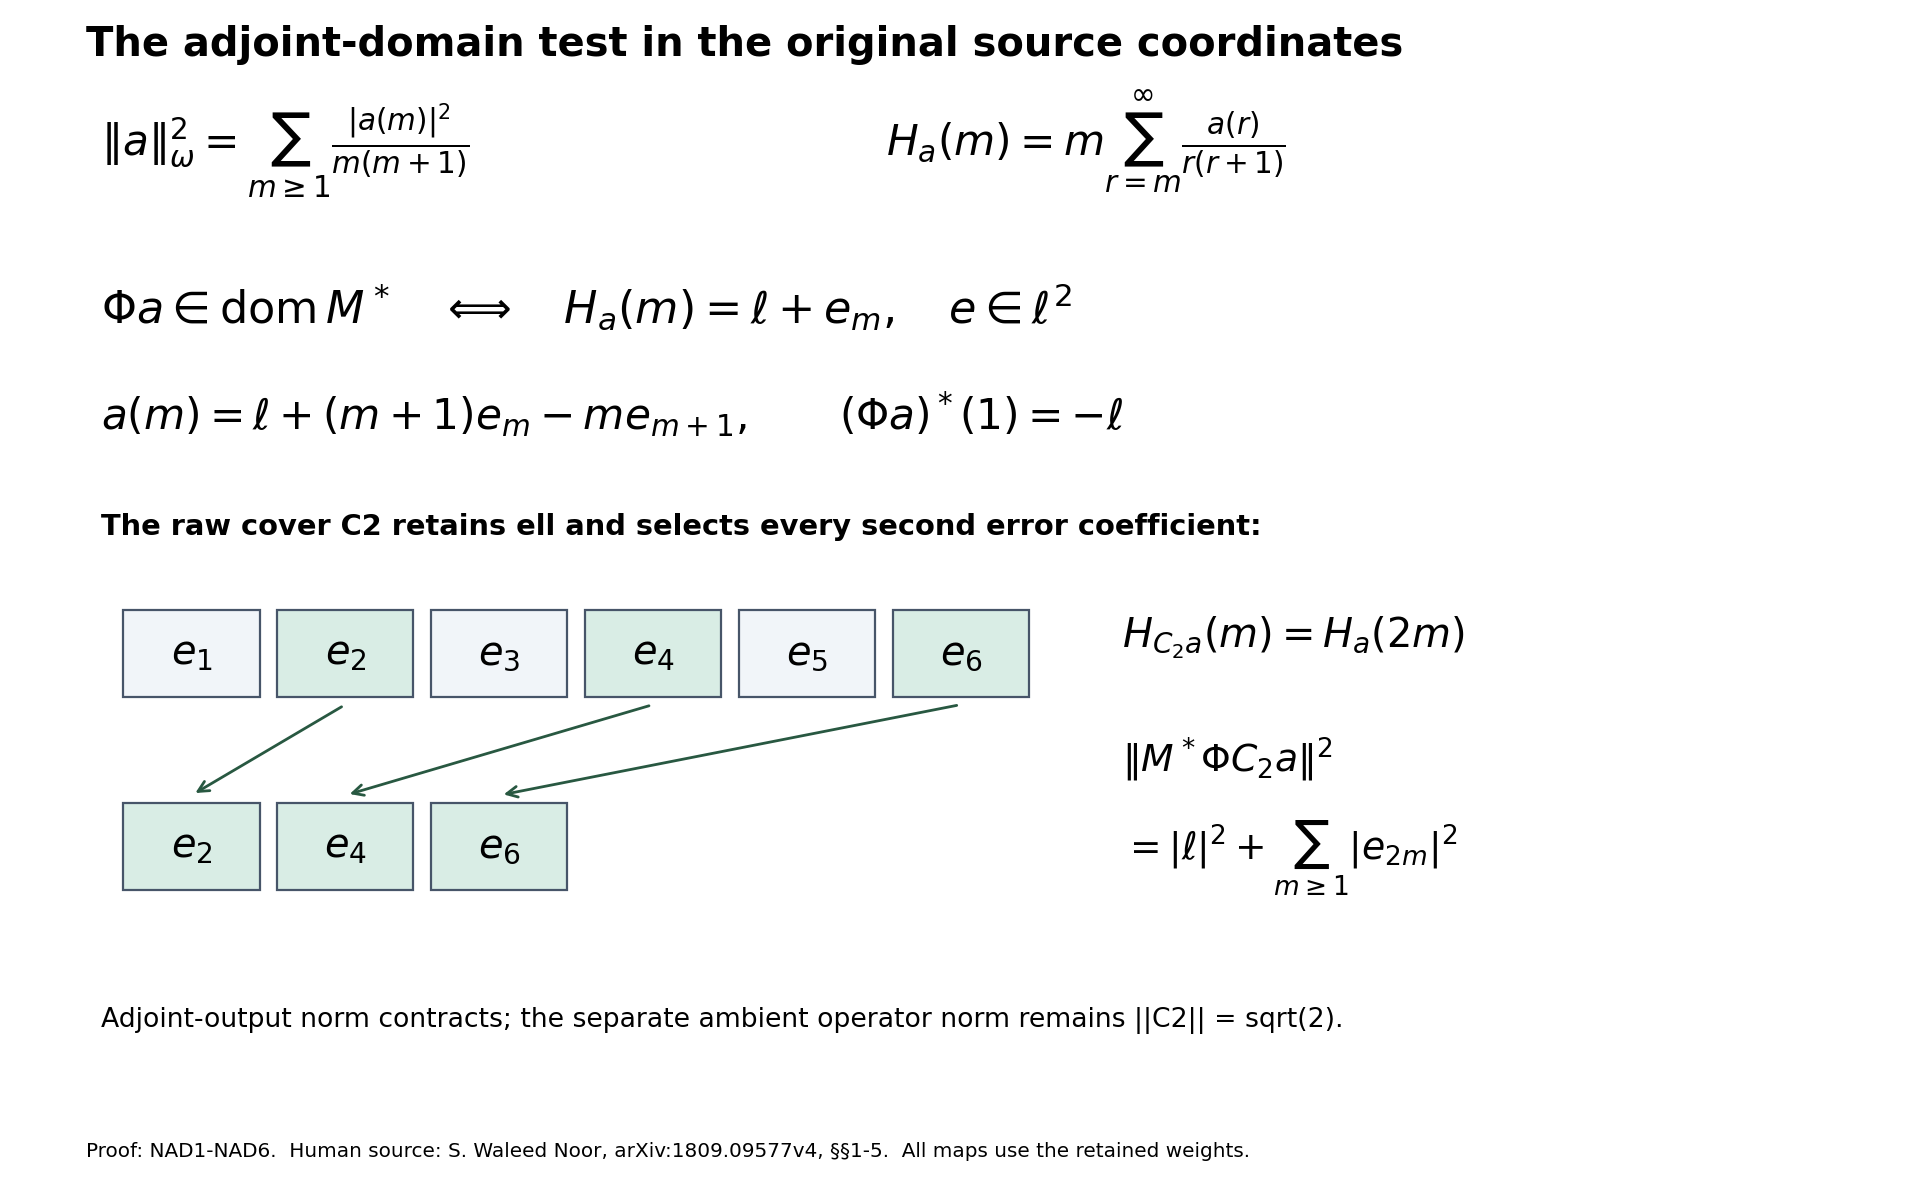
\includegraphics[keepaspectratio,alt={Weighted source-domain test and exact raw-cover subsampling}]{source_adjoint_domain.png}}
\caption{Weighted source-domain test and exact raw-cover subsampling}
\end{figure}

Figure: NAD2--NAD5 give the exact weighted-tail map, unique
scalar/sequence parameterization, boundary sign and cover action. The
displayed n=2 coefficient selection illustrates an exact symbolic
operator, not numerical zero data. \texttt{draw\_domain\_pullback.py} is
the reproducible source; PNG and SVG are retained. The rendered PNG was
visually inspected for formula signs, labels and clipping. The ambient
norm and adjoint-output norm are both named, with their different
constants retained.
